\textbf{2.} (7 puntos)

\vspace{20px}
\textit{Solución:}
\\

\begin{enumerate}
[label=\alph*)]
    \item La ley de Kirchhoff, como se nos indica en el enunciado, nos dice que cuanta más radiación puede absorber un objeto, más radiación puede emitir.

    Por otro lado, el voltaje medido en la termopila, que luego se amplifica para ser medido en el voltímetro, es proporcional a la radiación que recibe.

    Enlazando estas dos ideas, concluimos que la cara que más radiación sea capaz de absorber, será la que tenga más capacidad de emitir radiación térmica, y por ello,
    marcará un valor $V_{th}$ mayor en el multímetro.

    Las superficies más oscuras y menos pulidas son las que menor porcentaje de radiación reflejan y mayor porcentaje absorben.
    De estas dos características, es más determinante la textura y el acabado que el color de la superficie. Observamos que tenemos
    por tanto dos grupos distintos de caras en el cubo de Leslie: menos pulidas (negra mate y blanca mate) y más pulidas (bronce brillo y pulido espejo).
    Este hecho se ve reflejado en las mediciones del voltaje, en las que los valores están agrupados de 2 en 2 (caras A y B en un grupo, y C y D en otro).

    Por todo lo anterior, la relación de caras del cubo de Leslie es la siguiente:
    \begin{itemize}
        \item Cara A: espejo pulido
        \item Cara B: bronce brillo
        \item Cara C: blanco mate
        \item Cara D: negro mate
    \end{itemize}


    \vspace{20px}
    \item En este apartado se nos pide, a partir de los datos medidos en el experimento, comprobar que se cumple la Ley de Stefan-Bolztmann
    para el cuerpo negro.

    Esta ley nos dice que la potencia de emisión de una superficie es proporcional a la cuarta potencia de su temperatura:

    \begin{equation*}
        P_{surface} = \epsilon \sigma A T^4
    \end{equation*}

    Para comprobar que esta relación se cumple para nuestros datos experimentales no necesitamos saber ni el valor de la superficie $A$,
    ni de la constante de Boltzmann $\sigma$, ni de la emisividad $\epsilon$. Para cualquier valor de $A$ o $\epsilon$ esta relación
    debe ser verdadera. Así mismo, los datos de $T_{ambiente}$, amplificación de la señal y distancia de la termopila al cubo
    son innecesarios para nuestro objetivo.

    También nos damos cuenta de que la ley de Boltzmann nos proporciona la potencia de radiación en vatios, y en el multímetro estamos tomando
    medidas en voltios. Existe, por tanto, una constante de proporcionalidad entre ambas magnitudes, pero este valor también
    es irrelevante para nuestra comprobación.

    Por último, se nos dice que para calcular la diferencia de potencia emitida por una superficie, debemos tener en cuenta la emisión a temperatura ambiente.
    Una vez más, podemos descartar esta consideración, ya que lo que estamos buscando es comprobar si existe una relación lineal
    entre el voltaje $V_{th}$ medido en el multímetro y la cuarta potencia de la temperatura $T$. El valor constante de $P_{ambiente}$
    que siempre mide la termopila no influye en este hecho.

    Una manera de comprobar que este ley se cumple es realizar una regresión lineal de los datos experimentales, y ver si los datos se ajustan bien o no
    a la ecuación de una recta $V_{th} = a \cdot T^4 + b$. Realizamos esto mismo con el siguiente código en Python:\\

    \begin{verbatim}
import matplotlib.pyplot as plt
from scipy import stats

# Creating dataset
temperature = [95, 90, 85, 80, 75, 70, 65, 60, 55, 50]
x = [(t + 273.15)**4 for t in temperature]
y = [0.600, 0.586, 0.555, 0.544, 0.524, 0.508, 0.492, 0.476, 0.461, 0.446]

slope, intercept, r, p, std_err = stats.linregress(x, y)

def myfunc(x):
  return slope * x + intercept

mymodel = list(map(myfunc, x))

plt.scatter(x, y)
plt.plot(x, mymodel, color='red', linestyle='--',
         label="$V_{th} = %s\;T^4 + %.3f$" % (slope, intercept))
font1 = {'family':'serif','color':'black','size':20}
font2 = {'family':'serif','color':'darkred','size':15}
plt.title("Relación lineal entre $V_{th}$ y $T^4$", fontdict = font1)
plt.xlabel("$T^4 (K^4)$", fontdict = font2)
plt.ylabel("$V_{th} (V)$", fontdict = font2)
plt.legend(loc="upper left")
plt.show()


    \end{verbatim}

    \begin{center}
        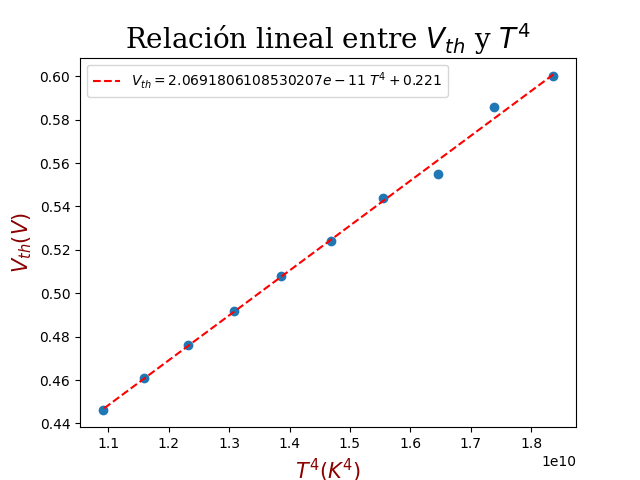
\includegraphics[scale=0.45]{files/img2}
    \end{center}


    Observamos que los datos se ajustan fielmente a una recta con pendiente $2,069 \times 10^{-11} V / K^4$.

    Como comprobación adicional, si consideramos que la emisividad del espejo pulido es $\epsilon = 0$, la medición
    de $0,383 V$ obtenida anteriormente debería originarse solo con la radiación de la temperatura ambiente. Si sustituimos
    el valor $273.15 + 26K$ en la ecuación de la recta obtenida por regresión lineal, el valor del voltaje obtenido es
    $0,387 V$, similar al obtenido experimentalmente.

    \vspace{20px}
    \item Un cuerpo negro es una idealización de un objeto físico, que absorbe toda la radiación incidente. En la realidad,
    los objetos físicos no son ideales. Los cuerpos grises son objetos físicos que absorben o emiten parcialmente radiación
    electromagnética para todas las longitudes de ondas.

    La relación entre la radiación térmica de un cuerpo gris y la radiación térmica de un cuerpo negro, a la misma temperatura,
    es la emisividad o emitancia del cuerpo gris.

    La emisividad del cuerpo negro es 1, y la del cuerpo gris es mayor que 0 y menor que 1.

    En nuestro experimento, si suponemos que la cara negra mate es un cuerpo negro ideal, con emisividad $\epsilon = 1$, y el
    espejo pulido tiene emisividad $\epsilon = 0$, tanto la cara blanca mate como la cara bronce brillo serán cuerpos grises,
    aunque la emisividad de la cara blanca mate será cercana a 1, y la de la cara bronce brillo será cercana a 0.

\end{enumerate}

